\documentclass[a4paper]{report}
\usepackage{graphicx}

\begin{document}
\title{baden - bloody accelerated digital emulation of neurons}
\author{Andreas Hartel}
\date{May 2015}
\maketitle

\chapter{Overview}
\begin{figure}
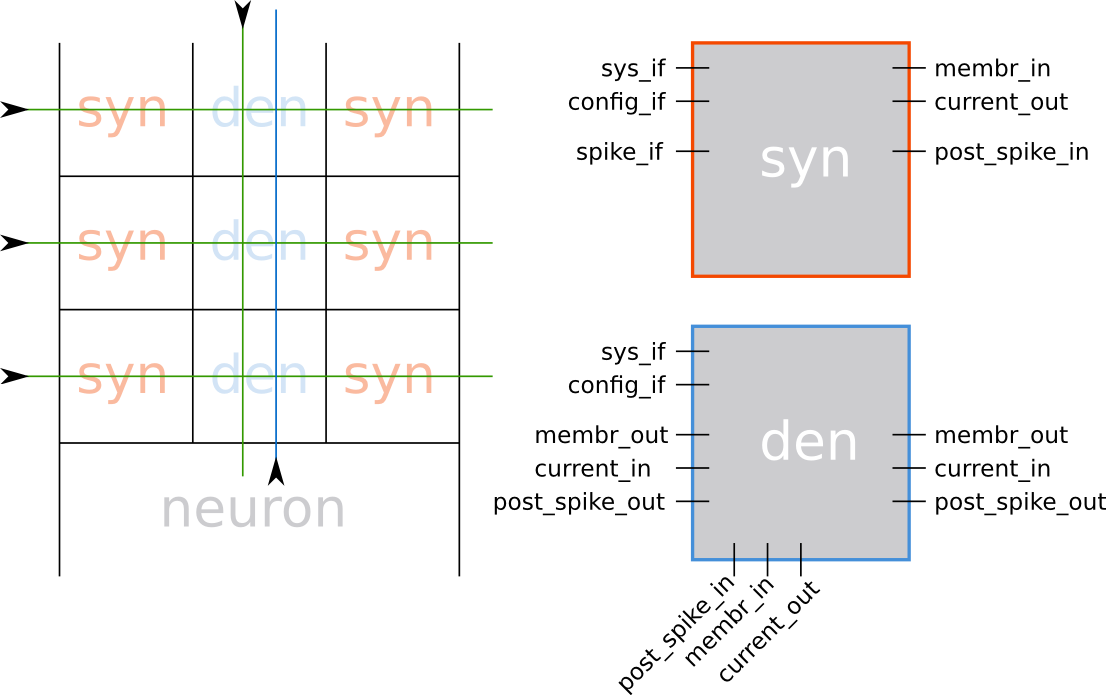
\includegraphics[scale=.6]{overview.png}
\end{figure}

\chapter{Implementation with rectangular conductance synapses}

\chapter{Implementation with exponential conductance synapses}
\section{Synapse}
\subsection{Ports}
	\begin{itemize}
		\item \texttt{input logic} $input_spike$
		\item \texttt{input fpType} $V_{mem}$
		\item \texttt{output fpType} $I_{out}$
	\end{itemize}
\subsection{Arithmetic elements}
\begin{itemize}
	\item MULTIPLIER for syn. conductance and syn. time constant
		\begin{equation}
			g_{syn}^{decay} = g_{syn} \cdot \tau_{syn}^{-1}
		\end{equation}
	\item SUBTRACTOR for diff. of reversal potential and membrane potential
		\begin{equation}
			V_{mem,rev}^{diff} = E_{rev} - V_{mem}
		\end{equation}
	\item MULTIPLIER of difference of potentials and momentary conductance
		\begin{equation}
			I_{syn} = g_{syn} \cdot V_{mem,rev}^{diff}
		\end{equation}
\end{itemize}
\subsection{Parameters}
\begin{tabular}{ll}
$E_{rev}$ & $A(9,6)$\\
$g_l^{jump}$ & $U(7,9)$\\
$\tau_{syn}^{-1}$ & $U(1,15)$\\
\end{tabular}
\section{Dendritic element}
\subsection{Ports}
	\begin{itemize}
		\item \texttt{input fpType} $I_{syn,0}$
		\item \texttt{input fpType} $I_{syn,1}$
		\item \texttt{input fpType} $I_{upper}$
		\item \texttt{input fpType} $V_{lower}$
		\item \texttt{output fpType} $I_{lower}$
		\item \texttt{output fpType} $V_{upper}$
		\item \texttt{output fpType} $V_{mem}^{syn0}$
		\item \texttt{output fpType} $V_{mem}^{syn1}$
	\end{itemize}
\subsection{Arithmetic elements}
\begin{itemize}
	\item ADDER for syn. currents from both synapses connecting to this element
		\begin{equation}
			I_{syn}^{tot} = I_{syn,0} + I_{syn,1}
		\end{equation}
	\item ADDER for sum of synaptic currents and current membrane potential
		\begin{equation}
			V_{mem}^{syn} = V_{mem} + I_{syn}^{tot}
		\end{equation}
	\item SUBTRACTOR for diff. of reversal potential and membrane potential
		\begin{equation}
			V_{mem,rev}^{diff} = E_l - V_{mem}
		\end{equation}
	\item MULTIPLIER of difference of potentials and membrane time constant
		\begin{equation}
			I_{leak} = \tau_{mem}^{-1} \cdot V_{mem,rev}^{diff}
		\end{equation}
	\item ADDER for membrane voltage (incl. syn. current) and leak current
		\begin{equation}
			V_{mem}^{syn,leak} = V_{mem}^{syn} + I_{leak}
		\end{equation}
	\item ADDER for membrane voltage so far and current from upper comp.
		\begin{equation}
			V_{mem}^{new} = V_{mem}^{syn,leak} + I_{in}^{upper}
		\end{equation}
	\item SUBTRACTOR for membrane voltage of this and the lower compartment
		\begin{equation}
			V_{comp}^{diff} = V_{mem} - V_{mem}^{lower}
		\end{equation}
	\item MULTIPLIER of diff. of comp. potentials and inter-comp. cond.
		\begin{equation}
			I_{out}^{lower} = V_{comp}^{diff} \cdot g_{int}
		\end{equation}
\end{itemize}
\subsection{Parameters}
\begin{tabular}{ll}
$E_l$ & $A(9,6)$\\
$\tau_{mem}^{-1}$ & $U(1,15)$\\
$g_{int}$ & $U(0,16)$\\
\end{tabular}
\end{document}
